\documentclass[journal]{IEEEtran}
\usepackage{amsmath,amssymb}
\usepackage{booktabs}
\usepackage{graphicx}
\usepackage{hyperref}
\usepackage{multirow}
\usepackage{xcolor}


% ---- Anonymization toggle: \anonymoustrue for review submission, \anonymousfalse for camera-ready ----
\newif\ifanonymous
\anonymoustrue

\ifanonymous
\newcommand{\repourl}{\url{https://anonymous.4open.science/status/moba-draft-policies}}
% Anonymized review mirror of the deployed web tool (single line to update):
\newcommand{\deployurl}{\url{https://draft-assistant-review.vercel.app}}
\else
\newcommand{\repourl}{\url{https://github.com/maxsegan/moba-draft-policies}}
\newcommand{\deployurl}{\url{https://www.hotsfever.com}}
\fi
% -----------------------------------------------------------------------------------------------------

\begin{document}

\title{Diagnosing and Repairing Out-of-Distribution\\ Failure in MOBA Draft Policies}
\ifanonymous
\author{Anonymous Authors}
\else
\author{Max~Segan, Ernest~Pysher, James~Frankel, and Hod~Lipson}
\fi
\maketitle

\begin{abstract}
In multiplayer online battle arena (MOBA) drafting, two teams alternately ban and pick heroes from a shared pool to build competing five-hero compositions, and a noisy match decides the winner. In Heroes of the Storm, a 90-hero pool spans $7.2 \times 10^{14}$ matchups; 1.95 million ranked drafts cover a vanishing, clustered fraction, so out-of-distribution behavior dominates policy quality. Search exploits learned value functions' out-of-distribution optimism, assembling structurally broken teams rated as competitive, and pessimistic offline reinforcement learning does not repair this: conservative and implicit Q-learning collapse to behavioral cloning, and mildly conservative Q-learning to a near-deterministic ten-hero policy. We decompose draft-policy quality into composition safety and interaction-awareness, with metrics that detect both collapses. We also report a pitfall in our own first pipeline: features built from aggregate statistics that contained each game's own outcome made the value function overconfident and inflated its reported accuracy and gains. With out-of-fold statistics, and with judges that share no data with any agent and are calibrated on real broken teams, the repair that works is search plus a structural mask. Monte Carlo tree search over a value function with domain features is interaction-aware, and a mask that removes any pick leaving no valid completion eliminates the broken teams search still builds, with a small gain in win probability. Synthetic training data for never-observed compositions also improves safety, but it dulls interaction-awareness, and we no longer recommend it. Search beats every behavior-anchored method under every independent judge (0.61 vs.\ 0.44--0.45 tournament win probability), while its gains from extra simulations and from domain features are smaller than the agents' own value function suggests. Code, models, and the in-browser agent are open-source.
\end{abstract}

\begin{IEEEkeywords}
MOBA drafting, team assembly, offline reinforcement learning, Monte Carlo tree search, out-of-distribution generalization.
\end{IEEEkeywords}

\section{Introduction}

Drafting has three properties that drive this paper: two opponents alternately claim discrete, rivalrous elements from a shared pool to assemble competing sets; the value of a set depends nonlinearly on interactions within it and against the opposing set; and a noisy downstream process decides the winner. Sports drafts share this structure but are rarely logged at scale. Drafting in multiplayer online battle arena (MOBA) games offers millions of logged episodes under fixed rules. In Heroes of the Storm (HotS), two teams of five alternate through 16 actions, banning 6 heroes and picking 10 from a pool of 90, before the match is played. HotS is in maintenance mode: a fixed 90-hero pool across 4.5 years of one major version gives an unusually stationary corpus. The draft matters: models that see only the completed draft predict outcomes at about 57\% on held-out games, a large edge in a balanced game.

Two properties make learned drafting hard. The first is coverage: roughly $7.2 \times 10^{14}$ final matchups ($\tfrac{1}{2}\binom{90}{5}\binom{85}{5}$), of which our 1.95 million drafts cover a vanishing and clustered fraction, so a policy must behave sensibly in states it has never observed. The second is evaluation: a completed draft only shifts the odds of the match, so the reward for training and search is itself a win probability model estimated from the same sparse data, and value and policy errors compound.

\begin{figure}[t]
\centering
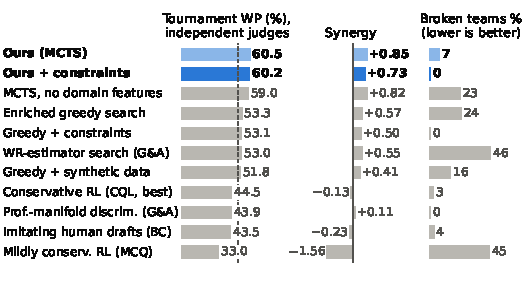
\includegraphics[width=\columnwidth,height=1.95in,keepaspectratio]{fig_glance_revision.pdf}
\caption{Results at a glance: the twelve-strategy round-robin (132 ordered pairs $\times$ 200 drafts; Section~\ref{sec:tournament}). First column: mean win probability under four composition-corrected judges that share no data with any agent (dashed line: 50\%); the CQL row shows the better variant per column. Anchoring to human behavior is safe but blind to interactions; greedy value search sees interactions but is unsafe; MCTS reaches both, and constraint masking removes its residual broken teams with a small gain in win probability.}
\label{fig:glance}
\end{figure}

Prior work treats draft outcome prediction and hero recommendation as supervised learning and reports held-out accuracy~\cite{chen2018drafting,gourdeau2021discriminative,summerville2016draft,lee2022draftrec}. That accuracy is a poor guide to policy quality. Three value functions within 0.2 percentage points of held-out accuracy (57.6--57.7\%) yield different greedy policies; the naive and enriched policies make the same pick at matched states only 8--9\% of the time. Under search, each model's behavior out of distribution decides policy quality: the optimizer finds states that are vanishingly rare in human play, such as five tanks or no healer, and the models score them as competitive. The evidence that such teams fail is visible only when heroes are grouped by role: the role-degenerate compositions players occasionally field consistently underperform.

The standard offline RL remedy is pessimism toward out-of-distribution actions~\cite{kumar2020conservative,lyu2022mildly}. With terminal reward and exact Monte Carlo returns, algorithmic pessimism reduces to behavioral anchoring (Section~\ref{sec:cql}). Conservative Q-Learning (CQL) cuts degenerate compositions to 0.4--3.6\% by collapsing to behavioral cloning (70--73\% agreement with the behavior policy, negative synergy), and Mildly Conservative Q-Learning (MCQ) collapses to a near-deterministic ten-hero policy. We therefore split draft quality into two axes. \textbf{Composition safety} asks whether a team has the structural roles it needs (healer, frontline, ranged damage). \textbf{Interaction-awareness} asks whether it responds to the opponent and exploits internal synergies. Safety is the easy axis, inherited by any method that stays near human behavior; no pessimism-based method we tested achieves interaction-awareness.

What achieves both is search plus a structural mask. AlphaZero-style Monte Carlo tree search (MCTS) over a value function with features built from role and outcome statistics finds interactions, and a hard mask that prunes structurally invalid picks removes the broken teams search still builds. Teaching the value function about broken teams with synthetic data, the repair our submission proposed, improves safety but dulls interaction-awareness (Section~\ref{sec:synth}). Building those statistics correctly matters. In our first pipeline they came from community aggregates that contained each game's own outcome, test games included. The leak inflated held-out accuracy, made the value function overconfident, and inflated its own measure of the gains from features and simulations. Independent judges confirm neither the feature gain nor any gain past 400 training simulations, and removing the leak does not change that (Sections~\ref{sec:leak} and~\ref{sec:mcts}). This revision rebuilds every value function on out-of-fold statistics and judges every agent with references that share no data with it. In a twelve-strategy tournament judged that way (Fig.~\ref{fig:glance}), MCTS agents lead at 0.61 win probability, greedy searchers follow at 0.51--0.54, and every behavior-anchored method trails at 0.44--0.45. Our contributions:
\begin{enumerate}
 \item A decomposition of draft quality into composition safety and interaction-awareness, with metrics (counter responsiveness, resilience, synergy, pick diversity, behavioral similarity) that separate compositional reasoning from mimicry. With them we show that CQL, BC-regularized CQL, and IQL reach safety by behavioral cloning and that MCQ's penalty does not transfer to this discrete setting.
 \item Role-composition heuristics that flag classes of compositions as bad despite their near-absence from game data (no-healer teams win 42\% in our corpus), used to evaluate policies, build features, and define a structural mask. We show that such statistics must be computed out of fold: in-sample statistics leak each game's outcome into its own features, and the value function becomes overconfident (calibration slope 0.78 vs.\ 0.99).
 \item A repair that reaches both axes: MCTS self-play over a value function with domain features, plus a structural mask. Under independent judges, MCTS beats every anchored and greedy baseline, including reimplementations of a published drafter and of an earlier win-rate estimator. At matched search, features change neither independent win probability nor the degenerate rate significantly (18.5\% vs.\ 13.9\% at 200 simulations); more simulations bring it to 6.6\% (4.6\% with argmax root). The mask guarantees 0\%, keeps positive synergy, and adds about 0.01 win probability, and the masked agent ties for first in the tournament. Synthetic data for unseen compositions, tested as an alternative, trades interaction-awareness for safety.
 \item An open-source systems stack:\footnote{\repourl} a fused CUDA MCTS kernel sustaining 140--161 episodes/second per GPU, 2.2$\times$ a tuned batched host pipeline at equal search quality (supplement), and an in-browser deployment of the full agent in a $\sim$20~MB download.
\end{enumerate}

\section{Background and Related Work}

\textit{Drafting.} Game-playing agents for MOBA and real-time strategy games focus on in-match control. OpenAI Five~\cite{berner2019dota} restricted Dota~2 to 17 heroes and drafted by exhaustive search; AlphaStar~\cite{vinyals2019grandmaster} has no draft. Draft-specific work falls into two camps. Outcome prediction estimates win probability and optionally searches against it: Chen et al.~\cite{chen2018drafting} used MCTS over a predictor in Dota~2, and JueWuDraft~\cite{chen2021juewudraft} scaled the recipe to Honor of Kings. Imitation reproduces expert selections: Summerville et al.~\cite{summerville2016draft} predicted professional picks with sequence models, Gourdeau and Archambault~\cite{gourdeau2021discriminative} drafted by minimizing a discriminator's distance to professional play, and DraftRec~\cite{lee2022draftrec} restricts recommendations to observed combinations. Imitation sidesteps out-of-distribution states at the cost of novel strategy. Gourdeau and Archambault conjectured that MCTS over a win-rate estimator would wander into poorly characterized compositions and proposed constraining search to the professional manifold. We confirm the failure (Section~\ref{sec:gap}), show that anchoring gives safety without interaction-awareness (Section~\ref{sec:cql}), evaluate the same author's released win-rate estimator (Section~\ref{sec:gourdeau}), and implement a structural version of the constraint (Section~\ref{sec:constrained}).

\textit{Offline RL and pessimism.} CQL~\cite{kumar2020conservative} pushes down Q-values of actions underrepresented in the data; MCQ~\cite{lyu2022mildly} penalizes only Q-values above a threshold; BEAR~\cite{kumar2019stabilizing} and TD3+BC~\cite{fujimoto2021minimalist} constrain the policy toward the behavior policy; IQL~\cite{kostrikov2022iql} avoids querying unseen actions. Levine et al.~\cite{levine2020offline} survey the area. We add structure through features and a rule-based mask instead.

\textit{Value functions under search.} Search amplifies the errors of its value function~\cite{silver2016mastering,silver2018general}, as in reward-model overoptimization~\cite{gao2023scaling}; here no terminal evaluation by rule exists, and the value function is learned from the data the policy must generalize beyond. Features built from outcome statistics add target leakage~\cite{kaufman2012leakage}: when a row's features include its own outcome, the model over-trusts them and is overconfident wherever the statistics lack the outcome, which includes every state search generates. The standard remedy is out-of-fold or ordered statistics~\cite{prokhorenkova2018catboost}. Our CUDA kernel differs from host-tree MCTS pipelines~\cite{chaslot2008parallel,wu2019accelerating} by running the whole episode, tree and networks, in one kernel launch.

\section{Problem Setup}
\label{sec:setup}

\subsection{Draft Formalization and Data}

A draft is 16 actions (6 bans, 10 picks) in a fixed order. The state holds multi-hot vectors of each team's picks and the bans, map (14), skill tier (3), step, and step type: 289 dimensions. Terminal reward is the game outcome. The behavior policy $\pi_\beta$ is our corpus of ranked Storm League replays, pinned in May 2026 and filtered to patch 2.55: 1,949,087 replays from December 2021 to May 2026, with the hero pool fixed at 90. Skill enters as three tier labels assigned by our collection pipeline from each game's average rank. Because of an off-by-one in that pipeline, the labels group ranks unevenly: low is Bronze (19.5\% of games), mid is Silver, Gold, and Master (48.4\%, including 0.3\% with no recorded rank), and high is Platinum and Diamond (32.1\%). The submission described them as Bronze--Gold, Platinum--Diamond, and Master. All models, statistics, and evaluations use the labels consistently, so they act as three fixed skill strata (the one exception is the submission's external composition table, keyed by Heroes Profile's own rank groups and read only by the submitted value functions); retraining the leak-free enriched and naive models with correct rank groupings (either the boundaries above or the site's Bronze--Silver, Gold--Platinum, Diamond--Master) moves held-out accuracy by at most 0.25pp and post-snapshot calibration slope by at most 0.07, and leaves the two models within 0.1pp of each other. These drafts come mostly from solo and duo queue, where players pick by preference and comfort, so $\pi_\beta$ reflects social habit as much as strategy. All models use team-swap augmentation. Splits are at the replay level: the test set is the submission's 38,981 replays, a 2\% hash-selected validation set (38,214) serves early stopping and seed selection, and 1,871,892 replays train (3.74M swap-augmented rows). Nothing retrained for this revision is selected on test data; the inherited baselines (the Gourdeau estimator, GD, CQL, IQL, MCQ, and the discriminator) keep the submission's checkpoints, which were selected on test accuracy.

\paragraph{Post-snapshot games} Our database kept collecting after the snapshot. We hold out 291,837 later games that no agent, value function, or agent statistic touched; they are used only to build the independent references (Section~\ref{sec:refs}): 153,739 snapshot-era games uploaded after the snapshot and 138,098 on the build in force at snapshot time (2.55.16.97039), with no balance change. A further 158,608 games on the 2.55.17 builds, after a balance patch, serve as a drifted check. No game from a build released after 2026-09-27 is used.

\subsection{Value Functions and Outcome Leakage}
\label{sec:leak}

\begin{table}[t]
\centering
\caption{Win probability models. Submitted: the original checkpoints and external statistics. Leak-free: retrained on out-of-fold statistics from our training split, early-stopped on validation; mean of 3 seeds (SD $\le$0.11pp). Test: the 38,981 held-out replays. Post: 291,837 post-snapshot games. Slope: calibration slope on Post (1 is calibrated, below 1 overconfident; 3-seed SD 0.02--0.08). On Test every leak-free model's slope exceeds 1 (1.12--1.22, naive included), a property of that sample, so we use Post. All rows 256$\to$128 MLP, dropout 0.3, AdamW; Gourdeau is a separately designed estimator (Section~\ref{sec:gourdeau}).}
\label{tab:models}
\setlength{\tabcolsep}{3.4pt}
\begin{tabular}{lccc|ccc|c}
\toprule
& \multicolumn{3}{c|}{Submitted} & \multicolumn{3}{c|}{Leak-free} & \\
Model & Test & Post & Slope & Test & Post & Slope & Dim \\
\midrule
Naive & 57.8 & 56.8 & 1.02 & 57.7 & 56.8 & 1.07 & 197 \\
Hero Str. & 57.7 & 56.6 & 1.00 & 57.6 & 56.6 & 1.05 & 209 \\
Enriched & 58.1 & 56.8 & 0.88 & 57.7 & 56.8 & 0.99 & 283 \\
Enr., in-sample & -- & -- & -- & 57.2 & 56.3 & 0.78 & 283 \\
Gourdeau & 56.5 & 55.7 & 0.87 & -- & -- & -- & 194 \\
\bottomrule
\end{tabular}
\end{table}

Table~\ref{tab:models} lists the win probability (WP) models. The naive model sees hero multi-hots, map, and tier; hero strength adds per-hero win rates; the enriched model adds 86 features: role counts (18), per-hero counter deltas against the opponents (50), team pairwise counter and synergy aggregates (4), team-average and map win-rate deltas (4), meta strength (4), draft diversity (2), and the empirical win rate of each team's sorted role composition (4), with a pessimistic 33\% default for compositions below 50 games.

\textit{The leak.} The submission computed these statistics from aggregates published by the community database our replays come from. Our replays make up a median 38--67\% of the games behind each hero statistic, so every game's features, test games included, contained its own outcome, most strongly in sparse pairwise cells. Removing each test game's own contribution drops the submitted enriched model from 58.1\% to 57.0\%; removing as many random training games changes nothing. Trained on rows whose features contained their own labels, the model learned to over-trust the pairwise features, and on games outside the statistics it is overconfident (post-snapshot slope 0.88 vs.\ 1.02 for the naive model).

\textit{The fix.} We now compute every statistic, including the composition table, from our own training split, out of fold: training rows in each of five hash folds get features from the other four folds; validation, test, post-snapshot rows, and every searched draft use statistics over the whole training split, which contain none of them. The external aggregates no longer enter any value function or judge trained for this revision; one inherited tournament baseline (CQL, enriched) still reads them. The leak-free enriched model is calibrated on unseen games (slope 0.99) and exactly as accurate as the naive model (57.7\% on test, 56.8\% post-snapshot). The same model with in-sample statistics loses half a point and is strongly overconfident (slope 0.78). The submitted 0.3pp accuracy edge came from the test games' own outcomes. We report held-out calibration slope for every value function and judge.

\textit{What the leak does to search.} To isolate the mechanism without balance drift we split the snapshot by hash into halves A and B, trained value functions on A, and judged search against them with references built only from B (supplement). With in-sample statistics a value function trained on 975K games reports 59.4\% on its own validation rows, reaches 56.1\% on B, and has slope 0.61; with out-of-fold statistics it reports 56.3\%, reaches 57.0\%, and has slope 1.10. Raising search from 1,024 to 16,384 simulations lifts the in-sample value function's own score by 0.068 and the B references by 0.035; the out-of-fold value function's own score (+0.061) and the B references (+0.052) move almost together. A small in-sample value function (122K games) shows classic over-optimization: its own score climbs to 0.93 while the B references stop improving after 4,096 simulations. Calibration slope flagged the problem; the disagreement of a seed ensemble sharing the same statistics did not.

\subsection{Evaluation}
\label{sec:eval}

\paragraph{Composition safety} Healer rate and degenerate rate: no healer, no frontline, no ranged damage, or 3+ heroes in one role. These are the classes that role-composition statistics show underperforming (no-healer teams win 42.4\% of 51,244 games in our training split) or absent from play.

\paragraph{Interaction-awareness} Pairwise deltas are observed win rates minus their independence expectation: the counter delta of $a$ against $b$ is $\mathrm{WR}(a\text{ vs }b) - [\mathrm{WR}(a) + (100 - \mathrm{WR}(b)) - 50]$, and the synergy delta of teammates is $\mathrm{WR}(a\text{ with }b) - [\mathrm{WR}(a) + \mathrm{WR}(b) - 50]$. \textit{Counter responsiveness} averages our heroes' counter deltas against the opponents, \textit{synergy} averages within-team synergy deltas, and \textit{resilience} scores each pick against the opponent's \textit{subsequent} picks, information no agent sees when choosing. Behavioral signals need no statistics: distinct heroes, pick entropy, top-10 concentration, and agreement with the behavioral-cloning model (GD similarity). The interaction metrics use the community aggregates as an evaluation instrument; no value function in this paper reads them. The two sources overlap in games, so some circularity between features and metrics remains. On 291,837 post-snapshot games, which the aggregates cannot contain, both metrics predict outcomes monotonically after controlling for team strength (+9.1pp synergy, +8.0pp counter, top vs.\ bottom decile; supplement).

\subsection{Independent References}
\label{sec:refs}

An agent cannot be graded by the value function it was trained or searched against. The submission's MCTS ``Avg WP'' and two of its four tournament judges did exactly that. The revision scores every generated draft with references that share no game, statistic, or search with any agent. \textit{gN}: the mean of three enriched judges trained with out-of-fold statistics only on the post-snapshot games, including a role-composition table built from those games. (A first version read the external composition table, which overlaps our corpus; the supplement compares the two.) \textit{gN-naive}: a hero-identity judge on the same games. \textit{RN}: a model-free realized-outcome index cross-fitted on the same games (hero win rates, synergy and counter residuals, and composition win rate from one half, weighted by a logistic fit on the other half). \textit{QM2026}, \textit{QM2021}: judges trained on Quick Match, a mode with no draft phase (116,589 and 91,365 games). On our test games, which none trained on, their held-out accuracy and calibration slope are 55.2\%/1.01 (gN), 56.0\%/0.91 (gN-naive), 54.7\%/1.04 (RN), 53.9\%/0.44 (QM2026), and 54.5\%/0.39 (QM2021). The Quick Match judges are overconfident on ranked drafts, so we read them for ordering. Each reference has a blind spot: gN shares our model class, RN cannot judge compositions nobody plays, and the QM judges have never seen a draft. The evidence is their agreement. The tournament consensus is the mean of gN, gN-naive, RN, and QM2026, fixed before any revised agent was scored. The composition correction below was added after every agent had been scored; the supplement reports all results without it.

\paragraph{Composition correction} A drafter that simply picks the highest win-rate heroes scored above every trained policy under a realized index, although 55\% of its teams were structurally broken. We therefore checked every reference on the 1.95M snapshot games, which none of them trained on. Real teams with no healer, no frontline, or three heroes of a stacking role (2.0\% of teams) win 4.9pp less often than RN predicts ($\pm$0.2), 5.0pp less than gN-naive, and 5.4pp less than QM2026; gN, which sees role counts, misses 3.0pp, and the consensus 4.6pp. RN's composition term shrinks each role multiset toward 50\% with a 200-game prior, and degenerate multisets hold a median of 2.5--10 games. The penalty does not come from who fields such teams: matchmaking gives them nearly equally skilled opponents, and controlling for causal per-player skill estimates and pick position moves it from $-$4.80 to $-$4.84pp. We correct each reference with three structure terms (no healer, no frontline, stacked role), fitted as a logistic adjustment to the reference's own held-out predictions on the post-snapshot games. On snapshot games the corrected references are calibrated on degenerate teams (consensus gap +0.0pp, each reference within 0.5pp) and on normal teams, with log loss equal or lower. Every number below uses the corrected references (supplement: audit, fits, and uncorrected values). The terms are learned from human degenerate teams, 93\% of which have one defect, as do 95--100\% of the MCTS agents' degenerate teams; a team nobody fields, such as five tanks, gets only the sum of its indicators.

\subsection{Search Methods}

\textbf{Greedy:} for each candidate hero, complete the draft with behavioral-cloning (GD) opponents trained on the snapshot (5 seeds), score the terminal state with the WP model, and pick the best. \textbf{GD:} the behavioral-cloning argmax. \textbf{CQL:} argmax of a conservatively learned Q-function. \textbf{MCTS:} an AlphaZero-style~\cite{silver2018general} policy-value network (Section~\ref{sec:mcts}); the benchmark of Table~\ref{tab:mcts} runs 200 simulations per move, and the tournament agents play the policy argmax with no search at decision time. All WP models are also checked on 28 hand-built sanity tests (absurd compositions, traps, symmetry).

\paragraph{Data availability} Raw replays cannot be redistributed under the Heroes Profile terms of service. Our corpus is a quota-limited subset of their public API's replay range, so the released repository includes the replay-id list, split and fold assignments, and the code that rebuilds every statistic from those replays.

\section{The Composition Gap}
\label{sec:gap}

\begin{table}[t]
\centering
\caption{Greedy cross-evaluation (480 drafts per drafter, leak-free 256$\to$128 models). Left: mean WP assigned by the column model (bold: self-evaluation); Ind.: mean of the four consensus references. Right: composition rates. Naive-vs-enriched healer difference 17.7pp ($p < 10^{-8}$).}
\label{tab:crosseval}\label{tab:comp}
\setlength{\tabcolsep}{3.3pt}
\begin{tabular}{lcccc|ccc}
\toprule
Drafter & Naive & H.~Str. & Enr. & Ind. & Heal\% & Rng\% & Deg\% \\
\midrule
Naive & \textbf{.640} & .626 & .617 & .570 & 61.3 & 79.4 & 58.5 \\
Hero Str. & .621 & \textbf{.640} & .612 & .569 & 77.1 & 76.5 & 49.4 \\
Enriched & .613 & .611 & \textbf{.641} & .571 & 79.0 & 76.5 & 50.2 \\
\bottomrule
\end{tabular}
\end{table}

\paragraph{Cross-evaluation} Each greedy drafter scores highest under its own model (Table~\ref{tab:crosseval}): search optimizes the specific model's value landscape. The enriched drafter gives up 2.7pp of naive-scored WP for a composition profile only its own model rewards, and the independent references do not rank the three drafters apart (0.569--0.571). All three fail composition safety. Healer rate rises with feature richness (61\% $\to$ 77\% $\to$ 79\%), while the degenerate rate falls from 58.5\% to about 50\% at the hero-strength step and then stays flat.

\begin{table}[t]
\centering
\caption{Main effect of each feature group on accuracy (with minus without, pp), from a $2^{10-3}$ resolution-V fractional factorial (128 models, leak-free statistics, 256$\to$128, seed 42). Main effects are unaliased with each other and with two-factor interactions; SE 0.02pp (test), 0.01pp (post). Submitted: the full-factorial marginal reported with leaky statistics.}
\label{tab:sweep}
\setlength{\tabcolsep}{4pt}
\begin{tabular}{lccc}
\toprule
Group & Test & Post & Submitted \\
\midrule
role counts & +0.10 & +0.14 & +0.16 \\
pairwise counters & +0.08 & +0.05 & +0.20 \\
map delta & +0.01 & +0.04 & +0.09 \\
pairwise synergies & $-$0.02 & +0.01 & +0.15 \\
map type & +0.00 & $-$0.01 & +0.01 \\
team average WR & $-$0.03 & $-$0.03 & $-$0.05 \\
synergy detail & $-$0.09 & $-$0.04 & +0.16 \\
counter detail & $-$0.06 & $-$0.06 & +0.14 \\
hero-map WR & $-$0.10 & $-$0.09 & $-$0.02 \\
hero WR & $-$0.11 & $-$0.13 & $-$0.16 \\
\bottomrule
\end{tabular}
\end{table}

\paragraph{Accuracy does not predict policy} A fractional factorial over ten feature groups (Table~\ref{tab:sweep}; the submission trained all 4,096 subsets with leaky features) shows that accuracy has stopped discriminating between feature sets: the 128 models span 57.0--58.0\% on test, and no group's main effect exceeds 0.14pp. Role counts, which read no statistics, have the largest effect. The four pairwise groups each lose 0.12--0.25pp against the submission, which is where self-inclusion was concentrated. The policy consequences of the same features are large. The leak-free models rate five tanks against a standard team at 0.31 (naive), 0.25 (enriched), and 0.08 after synthetic augmentation. Naive and enriched greedy policies agree on only 16\% of bans and 8--9\% of picks at matched states. Of the 50 drafts the naive model rates most above the enriched model, 68\% have no healer and 82\% are degenerate.

\paragraph{Independent baseline}
\label{sec:gourdeau}
We evaluate the HotS win-rate estimator released by Gourdeau, trained on our snapshot for the submission (the same checkpoint),\footnote{\url{https://github.com/HairyBlob/HotS-Drafter}} a Siamese network (994K parameters) with multiplicative map conditioning over multi-hot inputs, originally reported at about 61\% on contemporaneous data. On our snapshot it reaches 56.5\% (55.7\% post-snapshot), 1.2pp below our naive model. It rates five tanks at 45.5\%, nearly competitive, and under greedy search fields 41\% degenerate teams (Table~\ref{tab:rich}). The pathology belongs to identity-only inputs.

\section{Synthetic Data: A Tradeoff}
\label{sec:synth}

With a 512$\to$256$\to$128 network, the enriched model yields 23.7\% degenerate teams under greedy search with GD-argmax rollouts. One cause is training concentration: over 95\% of training teams have a healer, and 126--146 of the 252 role compositions per tier have fewer than 50 games in our training split. The submission repaired this with synthetic records for each such unseen composition (100 per tier, 41K in all, outcomes drawn at an assigned 10\% win rate adjusted by pairwise statistics). Retrained leak-free, augmentation leaves accuracy unchanged (57.5\%) and improves every safety measure under greedy search: degenerate rate 23.7\% $\to$ 13.6\%, healer rate 82\% $\to$ 92\%, five-tank WP 0.27 $\to$ 0.08, and sanity tests 22 $\to$ 26 of 28 (supplement: assigned rates of 0--50\% and a 27-configuration scope sweep). It also dulls interaction-awareness. In the rich evaluation (Table~\ref{tab:rich}) the augmented greedy agent has fewer degenerate teams (21.1\% $\to$ 15.2\%) and lower synergy (+0.44 $\to$ +0.29) and counter responsiveness (+0.16 $\to$ +0.09), and it loses to the unaugmented agent head to head (0.486 $\pm$ 0.004). The structural mask (Section~\ref{sec:constrained}) also lowers measured synergy somewhat (greedy +0.44 $\to$ +0.37), but it removes every degenerate team, leaves the value function untouched, and wins head to head (0.512). We therefore report augmentation as a tested option with a tradeoff and use the mask as the repair.

\section{Pessimistic Offline RL Collapses}
\label{sec:cql}

\begin{table*}[t]
\centering
\caption{Rich evaluation (5 opponent-sampling seeds $\times$ 1000 drafts per strategy). Counter and synergy use the community aggregates for every row. Ent.: pick entropy (bits); T10: top-10 hero share; GD: agreement with the behavioral-cloning model. The anchored rows read no aggregate statistics except CQL (enr.), retrained here on out-of-fold features (early stopping on the validation split); greedy and MCTS rows use leak-free value functions. MCTS rows: the five F\_oof seeds (Section~\ref{sec:mcts}), policy argmax.}
\label{tab:rich}
\begin{tabular}{lcccccccc}
\toprule
Strategy & Heal\% & Deg.\% & Counter & Synergy & Dist. & Ent. & T10\% & GD\% \\
\midrule
GD baseline & 99.3 & 1.2 & $+$.06 & $-$.20 & 64 & 4.37 & 74.1 & 82.2 \\
G\&A discriminator & 100.0 & 0.0 & $+$.07 & $+$.09 & 53 & 3.96 & 83.3 & 50.8 \\
CQL $\alpha$=.5 (naive) & 99.9 & 3.6 & $+$.07 & $-$.19 & 67 & 4.52 & 69.9 & 70.4 \\
CQL $\alpha$=1 (naive) & 99.7 & 3.0 & $+$.07 & $-$.16 & 70 & 4.52 & 70.2 & 72.3 \\
CQL $\alpha$=.5 (enr.) & 99.8 & 0.4 & $+$.06 & $-$.19 & 66 & 4.44 & 71.1 & 71.0 \\
CQL $\alpha$=2 (enr.) & 99.9 & 2.1 & $+$.06 & $-$.18 & 67 & 4.47 & 72.3 & 73.3 \\
BC-CQL $\beta$=1 & 99.9 & 2.2 & $+$.06 & $-$.16 & 68 & 4.50 & 71.0 & 70.8 \\
IQL $\tau$=.9 $\beta$=3 & 99.8 & 2.1 & $+$.07 & $-$.15 & 66 & 4.51 & 70.5 & 71.4 \\
MCQ $\tau$=.5 & 100 & 45.4 & $+$.01 & $-$1.60 & 10 & 2.87 & 100 & 0.8 \\
\midrule
Gourdeau estimator (greedy) & 66.6 & 41.1 & $-$.05 & $+$.31 & 90 & 5.75 & 42.0 & 4.8 \\
Enriched (greedy) & 83.5 & 21.1 & $+$.16 & $+$.44 & 90 & 5.96 & 35.2 & 4.1 \\
Enr.+aug (greedy) & 90.4 & 15.2 & $+$.09 & $+$.29 & 90 & 6.04 & 34.1 & 4.8 \\
MCTS & 94.4 & 6.2 & $+$.09 & $+$.78 & 32 & 3.52 & 88.8 & 3.1 \\
Constrained MCTS & 100 & 0.0 & $+$.08 & $+$.63 & 36 & 3.52 & 89.3 & 4.0 \\
\bottomrule
\end{tabular}
\end{table*}

\paragraph{Setup} Each replay gives 16 transitions (62M with team swaps). The Q-network (324K parameters, 512$\to$256$\to$128 hidden layers) maps the 289-dim state to 90 Q-values with invalid actions masked. With terminal-only reward and fixed-length episodes, Monte Carlo returns ($\gamma = 1$) make the Q-target the game outcome, so CQL is supervised outcome regression plus a behavior penalty:
\begin{equation}
\mathcal{L} = \mathcal{L}_\text{BCE}(Q(s,a), y) + \alpha \big( \mathbb{E}_\mu[\log \textstyle\sum_a e^{Q(s,a)}] - \mathbb{E}_\mathcal{D}[Q(s,a)] \big)
\end{equation}
The penalty can only anchor toward the behavior distribution; the experiments measure how tightly. We sweep $\alpha \in \{0.1, 0.5, 1, 2, 5\}$, MCQ's threshold $\tau \in \{0.4,\dots,0.8\}$, BC-regularized CQL's $\beta \in \{0.1, 0.5, 1, 2\}$ (a discrete analogue of TD3+BC~\cite{fujimoto2021minimalist}), and a six-cell IQL grid~\cite{kostrikov2022iql}.

\paragraph{CQL looks safe} With naive features CQL reaches 93.0--99.9\% healer and 2.2--13.4\% degenerate across $\alpha$ (best at $\alpha = 2$: 99.8\%, 2.2\%), safer than any greedy value-search agent. From identity inputs alone it appears to subsume the feature and augmentation pipeline.

\paragraph{Rich evaluation shows collapse} CQL, BC-CQL, and IQL agree with the behavioral-cloning model on 70--73\% of picks, use 66--70 heroes with concentrated pick distributions, and have negative synergy ($-$0.15 to $-$0.19), the same profile as GD itself (Table~\ref{tab:rich}). Greedy and MCTS agents agree with GD under 5\% of the time, use the full pool or a chosen head of it, and have positive synergy (+0.29 to +0.78). Adding the 86 enriched features to CQL makes it slightly safer and changes nothing else; across three network sizes and five target-update rates the collapse signals hold (GD agreement 69--77\%; supplement). The IQL cells are statistically identical, with advantage weights at 0.998--0.999; since the IQL Q-network's held-out loss (0.6948) is above that of a constant ($\ln 2$), the near-zero advantages may reflect an unfit Q-function as well as the absence of intermediate reward. GD itself shows that safety was never the hard problem: 99.3\% healer with negative synergy.

\paragraph{MCQ collapses differently} MCQ's penalty does not transfer to sigmoid-bounded discrete Q-values. For $\tau \geq 0.6$ it is inactive and yields a narrow policy over the same $\sim$9 heroes; at $\tau = 0.6$ every unit of the last hidden layer is zero on 200,000 held-out states. At $\tau = 0.5$ it drives Q toward zero, and every unit of the second and third hidden layers is zero on those states, so the Q-values reduce to the output bias: a fixed hero ranking. The resulting policy uses 10 heroes, always takes a healer, and is 45.4\% degenerate from role stacking.

\paragraph{The professional-manifold discriminator} We implement Gourdeau and Archambault's non-GAN drafter~\cite{gourdeau2021discriminative}. It is the safest learned strategy (100\% healer, 0\% degenerate) and shows no interaction-awareness (synergy +0.09, 53 heroes). Each of these methods reaches safety by anchoring to observed play. CQL's penalty treats every uncommon action alike: it cannot tell a fifth tank from a niche counter-pick whose matchup is rarely seen.

\section{MCTS with the Leak-Free Value Function}
\label{sec:mcts}

\paragraph{Training} The network (4.4M parameters) shares a residual backbone (289 $\to$ 768, 3 blocks, $\to$ 256) between a perspective-invariant policy head and a perspective-aware value head. In self-play it drafts one side with MCTS against a pool of 5 GD opponents. BC opponents keep trajectories near the WP model's training distribution and match the deployed setting, at the cost of exploitability by an adaptive opponent. WP evaluation and value head are symmetrized across team order. The submission trained 13 configurations (15 seeds each) against its leaky value functions. The revision adds B\_oof, F\_oof, and J\_oof: 200, 400, and 800 simulations per move against the leak-free enriched model, with its statistics in the kernel's lookup tables, five seeds each.

\paragraph{Benchmark} Each checkpoint drafts one side of the same 1,000 configurations (mid label, random map and side) against the GD pool with 200 simulations per move and its own value function at the leaves. We benchmark the first five seeds of each submitted configuration and every leak-free seed; no seed is selected. Within a run, the training worker keeps the checkpoint with the best periodic evaluation under the run's own value function, the submission's rule, which favors checkpoints that score well under that value function. Every draft is scored by the independent references. ``Train WP'' is the value function the configuration optimized: the submission's only reported metric.

\begin{table}[t]
\centering
\caption{MCTS benchmark (5 seeds $\times$ 1,000 drafts, 200 simulations at inference, root temperature 1). Train WP: the enriched value function the configuration optimized ($^\ast$: scored by the submitted enriched model, which that configuration did not optimize). gN, RN, QM26: composition-corrected references (Section~\ref{sec:refs}); gN seed SE 0.001--0.005 (M2: 0.016, one failed seed). C\_large doubles the backbone width, D\_deep deepens the policy head, H uses the augmented WP model, M2/N2 use relational-only and absolute-only feature subsets, K none; A\_partial and G\_base use step-conditioned value functions with and without enriched features (synergy not recomputed).}
\label{tab:mcts}
\setlength{\tabcolsep}{2.8pt}
\small
\begin{tabular}{lrccccrc}
\toprule
Config & Sims & Train & gN & RN & QM26 & Deg\% & Syn. \\
\midrule
\multicolumn{8}{l}{\textit{Submitted (leaky) value function}} \\
B\_fullwp & 200 & .721 & .639 & .610 & .635 & 15.0 & +1.14 \\
F\_400sim & 400 & .758 & .664 & .630 & .648 & 6.6 & +1.35 \\
I\_600sim & 600 & .766 & .656 & .625 & .650 & 7.8 & +1.44 \\
J\_800sim & 800 & .769 & .658 & .626 & .650 & 7.2 & +1.40 \\
E\_1M (1M ep.) & 200 & .753 & .661 & .629 & .653 & 7.3 & +1.34 \\
K\_truebase & 200 & .709$^\ast$ & .654 & .624 & .646 & 18.5 & +1.09 \\
C\_large & 200 & .738 & .653 & .619 & .641 & 6.6 & +1.27 \\
D\_deep & 200 & .659 & .612 & .586 & .614 & 6.4 & +0.34 \\
H\_augm. & 200 & .730$^\ast$ & .651 & .619 & .637 & 12.3 & +1.16 \\
M2\_relat. & 200 & .717$^\ast$ & .638 & .612 & .632 & 12.2 & +1.15 \\
N2\_abs. & 200 & .717$^\ast$ & .649 & .616 & .632 & 21.2 & +1.21 \\
A\_partial & 200 & .721$^\ast$ & .651 & .618 & .633 & 16.7 & -- \\
G\_base & 200 & .672$^\ast$ & .629 & .609 & .630 & 18.4 & -- \\
\midrule
\multicolumn{8}{l}{\textit{Leak-free value function}} \\
B\_oof & 200 & .698 & .652 & .620 & .640 & 13.9 & +1.13 \\
F\_oof & 400 & .716 & .666 & .632 & .649 & 6.6 & +1.26 \\
J\_oof & 800 & .728 & .655 & .624 & .648 & 11.1 & +1.34 \\
\bottomrule
\end{tabular}
\end{table}

\paragraph{Simulation scaling} Under the value function the submitted agents optimized, more training simulations help monotonically, 0.721 $\to$ 0.769 from 200 to 800 (+0.048). A judge is a noisier model than that value function, so even an honest gain shrinks under it. On the test replays, gN moves 0.48 per unit of the submitted value function and 0.56 per unit of the leak-free one (consensus 0.50 and 0.58; supplement), which sets the gain a judge should see without over-optimization. From 200 to 400 simulations the submitted agents' own score rises by 0.037, which predicts +0.018 under gN; gN rises by 0.025 ($\pm$0.005) and RN by 0.020, so this step transmits fully. From 400 to 800 the own score rises by 0.011 while gN falls by 0.006 ($\pm$0.002) and RN by 0.004: over-optimization. Synergy, which reads statistics that overlap the value function's, keeps rising. The leak-free pipeline behaves the same way. From 200 to 400 its own score rises by 0.018, gN by 0.013 ($\pm$0.003; predicted 0.010), and RN by 0.011. From 400 to 800 its own score rises by 0.012 ($\pm$0.004), while gN falls by 0.011 ($\pm$0.003) and RN by 0.008 ($\pm$0.003), gN-naive and QM2026 stay within noise, and the degenerate rate rises from 6.6\% to 11.1\%. At matched simulations leak-free and leaky agents score the same under independent references (F\_oof $-$ F\_400sim: gN +0.002), consistent with the submitted value function being only mildly leaky (slope 0.88). The leak therefore inflated the self-reported gains, and it does not explain the plateau past 400 simulations, which appears in both pipelines. A within-snapshot split experiment predicted that out-of-fold statistics would let more simulations keep paying off (supplement); at paper scale they do not. A value function calibrated on human games is not thereby calibrated on the drafts search produces. Three of the five J\_oof seeds were paused by a compute cap and resumed from their best-evaluation checkpoints (51K, 51K, and 107K episodes) without their replay buffers; the two uninterrupted seeds alone give gN $-$0.016 ($\pm$0.002).

\paragraph{Training length and root selection} Training for 1M episodes (vs.\ 300K) at 200 simulations helps under every reference (gN +0.022, RN +0.019, QM2026 +0.019) and halves the degenerate rate. E\_1M and F tie as the best configurations. Taking the argmax of root visit counts at inference adds 0.000--0.006 gN over sampling at temperature 1 (mean +0.003) and never lowers gN. Our benchmark operating point is F\_oof with argmax root (the tournament plays the policy argmax without search). F\_oof beats J\_oof under gN and RN and ties it under the other references, at half the training compute.

\paragraph{Features} The submission reported that enriched features add +0.023 WP over the identical featureless agent K\_truebase ($p < 0.001$), judged by the enriched agent's own value function. Under independent references the sign reverses: gN $-$0.015 ($\pm$0.005), RN $-$0.014, QM2026 $-$0.011. With leak-free features at matched search the difference is zero within error (gN $-$0.002 $\pm$ 0.003, RN $-$0.003 $\pm$ 0.003). The safety difference at matched search is not significant either: 13.9\% (B\_oof) vs.\ 18.5\% (K\_truebase) degenerate teams, $-$4.6 $\pm$ 3.5pp across seeds ($-$0.8 $\pm$ 4.6pp with argmax root). The drop to 6.6\% (4.6\% with argmax root) at the operating point comes mainly from doubling the simulations, which we did not run without features. The composition correction charges K\_truebase for its broken teams, but it also charges the sampled GD opponents, 12--13\% of whose teams are degenerate, so it moves the 200-simulation feature gaps by at most 0.003 under any reference. The submission's decomposition of the +0.023 gap into relational and absolute parts is withdrawn with it; under gN the absolute-only model (0.649) outscores the full model (0.639), and the relational-only model's 0.638 includes one failed seed (0.574; the other four average 0.654). A wider backbone (C\_large) is better than the base network under gN (+0.014) and safer; a deeper policy head (D\_deep) is worst under every reference.

\subsection{Round-Robin Tournament}
\label{sec:tournament}

Twelve strategies play every ordered pair for 200 drafts (both first-pick assignments, stratified maps and tiers; 132 pairs): MCTS and constrained MCTS, enriched, enriched+augmented, and constrained greedy, K\_truebase, the Gourdeau estimator and the G\&A discriminator, CQL (naive and enriched), GD, and MCQ. Agents were fixed before any tournament score existed. Value-function agents use leak-free models, except the inherited CQL (enriched) agent, which keeps the submission's checkpoint and external statistics. Both MCTS agents use the five F\_oof seeds, pooled (draft $i$ uses seed $i \bmod 5$); we chose F over J because the benchmark of the submitted configurations, scored by the same independent references, showed no gain beyond 400 simulations. K\_truebase pools its 15 seeds. Pairs among the six unchanged baselines reuse the submission's drafts. No contestant's value function is a judge.

\begin{table}[t]
\centering
\caption{Tournament: mean win probability over each strategy's 22 ordered pairs, and pairs won under the consensus (mean of gN, gN-naive, RN, QM2026; SE 0.001, clustered by draft configuration, without seed-to-seed variation of the agents). $^\dagger$Submission's checkpoint with external statistics. All judges composition-corrected (Section~\ref{sec:refs}). Deg.: degenerate rate of the strategy's teams.}
\label{tab:tourn}
\setlength{\tabcolsep}{1.8pt}
\small
\begin{tabular}{lcccccccc}
\toprule
Strategy & Cons. & Won & gN & RN & QM26 & QM21 & Deg. & Syn. \\
\midrule
Constr.\ MCTS & .610 & 21 & .617 & .606 & .595 & .690 & 0.0 & +.73 \\
MCTS & .610 & 21 & .613 & .599 & .604 & .699 & 7.3 & +.85 \\
MCTS, no feat. & .586 & 18 & .585 & .573 & .597 & .698 & 23.4 & +.82 \\
Constr.\ greedy & .538 & 16 & .542 & .538 & .520 & .497 & 0.0 & +.50 \\
Enr.\ greedy & .528 & 14 & .530 & .525 & .512 & .488 & 24.1 & +.57 \\
Enr.+aug greedy & .518 & 10 & .523 & .517 & .501 & .480 & 16.1 & +.41 \\
Gourdeau est. & .512 & 12 & .508 & .499 & .511 & .493 & 46.0 & +.55 \\
CQL enr.$^\dagger$ & .452 & 5 & .447 & .455 & .470 & .435 & 3.2 & $-$.16 \\
CQL naive & .448 & 5 & .444 & .451 & .470 & .448 & 4.5 & $-$.13 \\
G\&A discrim. & .447 & 5 & .446 & .445 & .477 & .444 & 0.0 & +.11 \\
GD & .441 & 5 & .436 & .446 & .463 & .427 & 3.5 & $-$.23 \\
MCQ & .310 & 0 & .310 & .347 & .279 & .202 & 45.1 & $-$1.56 \\
\bottomrule
\end{tabular}
\end{table}

Three tiers separate under every reference (Table~\ref{tab:tourn}): MCTS agents at 0.59--0.61, searching greedy agents at 0.51--0.54 (the Gourdeau estimator, the one external baseline that searches a value function, among them), and every behavior-anchored method at 0.44--0.45, with MCQ last. Rank correlation with the consensus over all twelve strategies is 0.94--0.99 for every reference, both Quick Match judges included, which share no game with any model here. Within the top six the Quick Match judges agree less (0.83): QM2021 places the greedy agents below 0.5. They confirm that searching a value function beats anchoring to human behavior; they leave the finer ordering among searchers open. Before the composition correction the Gourdeau estimator (46\% degenerate) scored 0.531, above the augmented greedy agent, and each constrained agent trailed or tied its unmasked version. MCTS beats K\_truebase head to head (0.559 $\pm$ 0.004; gN 0.565, RN 0.554, QM2026 0.530, QM2021 0.487), a comparison confounded by F\_oof's doubled simulation budget; at matched budget the benchmark shows no difference. Their degenerate rates differ more (7.3\% vs.\ 23.4\% of tournament teams), but that difference mixes features with the simulation budget in the same way.

\subsection{Structural Constraint Masking}
\label{sec:constrained}

Gourdeau and Archambault proposed constraining win-rate search to viable compositions~\cite{gourdeau2021discriminative}. We implement a structural version, which is our recommended repair: at each of our picks, a hero is masked out iff picking it would leave no completion from the remaining pool with at least one healer, one frontline, and one ranged-damage hero and at most two heroes per stackable role (decided exactly by memoized enumeration). The mask prunes only the invalid region, by rule, and guarantees 100\% healer and 0\% degenerate teams. Interaction-awareness survives it: constrained MCTS keeps synergy +0.63 (+0.78 unmasked) and the same pick entropy (3.52 bits), and masked greedy keeps +0.37, while the anchored methods of Table~\ref{tab:rich} sit at $-$0.15 to $-$0.20. The mask costs no win probability and gains a little: head to head with the same checkpoints, constrained MCTS scores 0.509 $\pm$ 0.003 against unconstrained MCTS, and masked greedy 0.512 $\pm$ 0.003 against unmasked greedy. Under the uncorrected references both pairs tied (0.499, 0.500), because those references barely charged the broken teams the mask removes.

\section{Discussion}
\label{sec:discussion}

\begin{figure}[t]
\centering
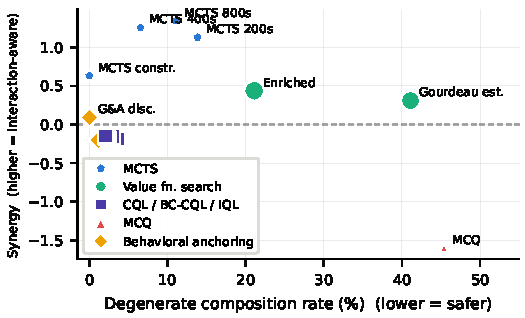
\includegraphics[width=\columnwidth,height=2.05in,keepaspectratio]{fig_safety_context_revision.pdf}
\caption{Safety vs.\ interaction-awareness (Table~\ref{tab:rich}; MCTS 200s/400s/800s are the leak-free configurations of Table~\ref{tab:mcts}, searched at inference with root temperature 1, while constrained MCTS is the policy argmax of Table~\ref{tab:rich}; anchored points are the submission's rich-evaluation runs). Marker size encodes hero diversity. Only MCTS reaches both low degenerate rate and positive synergy; masking pins the degenerate rate at zero.}
\label{fig:scatter}
\end{figure}

\paragraph{Two axes} Anchoring to human behavior provides safety, and a rule-based mask makes it exact (Fig.~\ref{fig:scatter}). Interaction-awareness requires searching a value function; no anchored variant reaches it. Some findings depend only on the problem structure. Any assembly domain separates structural validity from responsiveness to the opposing set. Any terminal-reward assembly problem trained with Monte Carlo returns leaves pessimism only the anchoring pathway. Validity masking applies wherever the invalid region can be described by rule. The interaction metrics port too, needing only pairwise outcome statistics and a reference behavior policy. The role taxonomy, the features, and the composition heuristics must be rebuilt per domain.

\paragraph{Practical lessons} Low degenerate rates in offline RL can mean behavioral cloning; report action diversity next to reward. Anchoring is a limitation here because $\pi_\beta$ reflects comfort-driven queue habits; where the behavior policy is near-optimal, staying near it is the right goal. Anyone building a value function from aggregate outcome statistics and then searching it should compute the statistics out of fold, check calibration on games outside them, and judge the policy with references the search never saw. In our submitted pipeline the leak cost half a point of accuracy, was invisible on a leaky test set, and inflated the value function's own measure of every gain; independent references confirm neither the feature gain nor any gain past 400 simulations, in either pipeline. Where invalid compositions can be described by rule, mask them during search: in our experiments a mask did better than teaching the value function about them with synthetic data, which also dulled interaction-awareness. The deployed web tool\footnote{\deployurl} runs MCTS in-browser at 50--200 simulations per move. Open problems include the in-match talent stage and patch-driven non-stationarity.

\section{Conclusion}

In team assembly the state space is huge and the terminal evaluation must itself be learned from clustered data. In MOBA drafting, search exploits the out-of-distribution optimism of learned value functions to assemble broken teams, and algorithmic pessimism does not repair this: with Monte Carlo returns, CQL anchors to the behavior distribution, IQL reduces to behavioral cloning, and MCQ collapses to ten heroes. What works is search plus a structural mask: MCTS self-play over a value function with domain features finds interactions, and the mask removes the broken teams search still builds. Synthetic data for unseen compositions improves safety but dulls interaction-awareness. Judged only by references no agent trained against, MCTS agents win 21 of 22 ordered matchups at 0.61 win probability, far above every anchored method (0.44--0.45), and the mask makes them valid by construction with a small gain. The first version of our pipeline built features from statistics containing each game's own outcome; measured by its own value function, deeper search and domain features added +0.048 and +0.023 win probability, while independent judges measured +0.018 and $-$0.015. Even with leak-free statistics, raising training simulations from 400 to 800 raised the agents' own score, lowered gN and RN by 0.008--0.011, and left the other references within noise. Value functions learned from aggregate outcomes and then searched should be built on out-of-fold statistics and checked for calibration; their agents should be scored by independent judges, and the simulation budget chosen against those judges. The judges need the same audit: ours under-charged real broken teams by about 5pp until we measured them on such teams.

\textit{Limitations.} One game. The independent judges are weaker than an in-corpus model (53.9--56.0\% vs.\ 57.7\% held-out) and each has a blind spot (Section~\ref{sec:refs}); their agreement is strong for the coarse ordering and weaker among searching agents. Their composition terms are fitted on human teams with one missing role, so they extrapolate to rarer structures, and the fitted penalty is about 2pp too large on games after the 2.55.17 balance patch. Post-snapshot games differ from the corpus in population, though not in patch. Tournament agents play the MCTS policy without search, and all agents trained against behavioral-cloning opponents, so exploitability by adaptive opponents is untested. The leak-free MCTS runs have five seeds (SE resolves about 0.01). Earlier in-sample checks of the agent's favorite hero combinations did not replicate on later games and are withdrawn. On 11,034 drafts from an amateur league with persistent five-player teams (supplement), whose games are in neither our corpus nor the aggregates, the leak-free enriched model drops from 57.7\% to 55.5\%, the same drop as the naive model; the shift re-weights familiar compositions (99.98\% fall in role compositions seen on the ladder). A blinded expert study and forward evaluation in an amateur league are in progress.

\ifanonymous
\section*{AI Disclosure}

Portions of this manuscript's text were drafted and edited with Claude (Anthropic)~\cite{claude}; all experiments, analyses, and claims were designed, verified, and approved by the authors.
\else
\section*{Acknowledgment}

We thank Heroes Profile (heroesprofile.com), whose API supplied both our replay corpus and the aggregate statistics. Heroes of the Storm is a trademark of Blizzard Entertainment. Portions of this manuscript's text were drafted and edited with Claude (Anthropic)~\cite{claude}; all experiments, analyses, and claims were designed, verified, and approved by the authors.
\fi

\section*{Conflicts of Interest}

The authors declare no conflicts of interest.

\begin{thebibliography}{20}

\bibitem{kumar2020conservative}
A.~Kumar, A.~Zhou, G.~Tucker, and S.~Levine, ``Conservative Q-Learning for Offline Reinforcement Learning,'' in \textit{Advances in Neural Information Processing Systems}, vol.~33, pp.~1179--1191, 2020.

\bibitem{levine2020offline}
S.~Levine, A.~Kumar, G.~Tucker, and J.~Fu, ``Offline Reinforcement Learning: Tutorial, Review, and Perspectives on Open Problems,'' \textit{arXiv preprint arXiv:2005.01643}, 2020.

\bibitem{kumar2019stabilizing}
A.~Kumar, J.~Fu, M.~Soh, G.~Tucker, and S.~Levine, ``Stabilizing Off-Policy Q-Learning via Bootstrapping Error Reduction,'' in \textit{Advances in Neural Information Processing Systems}, vol.~32, 2019.

\bibitem{chen2018drafting}
Z.~Chen, Y.~Sun, M.~Seif El-Nasr, and T.-H.~D.~Nguyen, ``The Art of Drafting: A Team-Oriented Hero Recommendation System for Multiplayer Online Battle Arena Games,'' in \textit{Proc. ACM Conf. Recommender Systems (RecSys)}, 2018.

\bibitem{gourdeau2021discriminative}
D.~Gourdeau and L.~Archambault, ``Discriminative Neural Network for Hero Selection in Professional Heroes of the Storm and DOTA 2,'' \textit{IEEE Trans. Games}, vol.~13, no.~4, pp.~380--387, 2021.

\bibitem{lee2022draftrec}
H.~Lee, D.~Hwang, H.~Kim, B.~Lee, and J.~Choo, ``DraftRec: Personalized Draft Recommendation for Winning in Multi-Player Online Battle Arena Games,'' in \textit{Proc. ACM Web Conf. (WWW)}, 2022.

\bibitem{summerville2016draft}
A.~Summerville, M.~Cook, and B.~Steenhuisen, ``Draft-Analysis of the Ancients: Predicting Draft Picks in DotA 2 using Machine Learning,'' in \textit{Proc. AAAI Conf. Artificial Intelligence and Interactive Digital Entertainment (AIIDE)}, vol.~12, no.~2, pp.~100--106, 2016.

\bibitem{chen2021juewudraft}
S.~Chen, M.~Zhu, D.~Ye, W.~Zhang, Q.~Fu, and W.~Yang, ``Which Heroes to Pick? Learning to Draft in MOBA Games with Neural Networks and Tree Search,'' \textit{IEEE Trans. Games}, vol.~13, no.~4, pp.~410--421, 2021.

\bibitem{lyu2022mildly}
J.~Lyu, X.~Ma, X.~Li, and Z.~Lu, ``Mildly Conservative Q-Learning for Offline Reinforcement Learning,'' in \textit{Advances in Neural Information Processing Systems}, vol.~35, 2022.

\bibitem{kostrikov2022iql}
I.~Kostrikov, A.~Nair, and S.~Levine, ``Offline Reinforcement Learning with Implicit Q-Learning,'' in \textit{Proc. Int. Conf. Learning Representations (ICLR)}, 2022.

\bibitem{silver2016mastering}
D.~Silver \textit{et al.}, ``Mastering the Game of Go with Deep Neural Networks and Tree Search,'' \textit{Nature}, vol.~529, no.~7587, pp.~484--489, 2016.

\bibitem{silver2018general}
D.~Silver \textit{et al.}, ``A General Reinforcement Learning Algorithm that Masters Chess, Shogi, and Go through Self-Play,'' \textit{Science}, vol.~362, no.~6419, pp.~1140--1144, 2018.

\bibitem{berner2019dota}
C.~Berner \textit{et al.}, ``Dota 2 with Large Scale Deep Reinforcement Learning,'' \textit{arXiv preprint arXiv:1912.06680}, 2019.

\bibitem{vinyals2019grandmaster}
O.~Vinyals \textit{et al.}, ``Grandmaster Level in StarCraft II using Multi-Agent Reinforcement Learning,'' \textit{Nature}, vol.~575, no.~7782, pp.~350--354, 2019.

\bibitem{fujimoto2021minimalist}
S.~Fujimoto and S.~S.~Gu, ``A Minimalist Approach to Offline Reinforcement Learning,'' in \textit{Advances in Neural Information Processing Systems}, vol.~34, 2021.

\bibitem{gao2023scaling}
L.~Gao, J.~Schulman, and J.~Hilton, ``Scaling Laws for Reward Model Overoptimization,'' in \textit{Proc. Int. Conf. Machine Learning (ICML)}, 2023.

\bibitem{chaslot2008parallel}
G.~M.~J.-B.~Chaslot, M.~H.~M.~Winands, and H.~J.~van~den~Herik, ``Parallel Monte-Carlo Tree Search,'' in \textit{Proc. Int. Conf. Computers and Games}, pp.~60--71, 2008.

\bibitem{wu2019accelerating}
D.~J.~Wu, ``Accelerating Self-Play Learning in Go,'' \textit{arXiv preprint arXiv:1902.10565}, 2019.

\bibitem{kaufman2012leakage}
S.~Kaufman, S.~Rosset, C.~Perlich, and O.~Stitelman, ``Leakage in Data Mining: Formulation, Detection, and Avoidance,'' \textit{ACM Trans. Knowledge Discovery from Data}, vol.~6, no.~4, pp.~15:1--15:21, 2012.

\bibitem{prokhorenkova2018catboost}
L.~Prokhorenkova, G.~Gusev, A.~Vorobev, A.~V.~Dorogush, and A.~Gulin, ``CatBoost: Unbiased Boosting with Categorical Features,'' in \textit{Advances in Neural Information Processing Systems}, vol.~31, 2018.

\bibitem{claude}
Anthropic, ``Claude (Fable 5),'' large language model, 2026.


\end{thebibliography}

\end{document}
